\chapter{Load, Performance and Stress Testing}

Load, performance, and stress testing are typically done to locate bottlenecks in a system, to support a performance-tuning effort, and to collect other performance-related indicators to help stakeholders get informed about the quality of the application being tested \cite{Sandler2004} \cite{Corporation2007}. 



The performance testing aims at verifying a specified system performance. This kind of test is executed by simulating hundreds of simultaneous users or more over a defined time interval \cite{DiLucca2006}. The purpose of this assessment is to demonstrate that the system reaches its performance objectives \cite{Sandler2004}. 


In a load testing, the system is evaluated at predefined load levels \cite{DiLucca2006}. The aim of this test is to determine whether the system can reach its performance targets for availability, concurrency, throughput, and response time. Load testing is the closest to real application use \cite{Molyneaux2009}. A typical load test can last from several hours to a few days, during which system behavior data like execution logs and various metrics are collected \cite{Afzal2009a}. 

The stress testing verifies the system behavior against heavy workloads \cite{Sandler2004}, which are executed to evaluate a system beyond its limits, validate system response in activity peaks, and verify whether the system is able to recover from these conditions. It differs from other kinds of testing in that the system is executed on or beyond its breakpoints, forcing the application or the supporting infrastructure to fail \cite{DiLucca2006} \cite{Molyneaux2009}.


While load testing is the process of assessing non-functional quality related problems under load. Performance testing is used to measure and/or evaluate performance
related aspects (e.g., response time, throughput and resource utilizations) of algorithms, designs/architectures, modules, configurations, or the overall systems. Stress tests puts a system under extreme conditions to verify the robustness of the system and/or detect various functional bugs (e.g., memory leaks and deadlocks) \cite{Afzal2009a}. The next subsections present details about the stress test process, automated stress test tools and the stress test results.

\subsection{Stress Test Process}

Contrary to functional testing, which has clear testing objectives, Stress testing objectives are not clear in the early development stages and are often defined later on a case-by-case basis. The Fig. \ref{fig:testprocess} shows a common Load, Performance and Stress test process  \cite{Jiang2010}.

\begin{figure}[!ht]
\centering
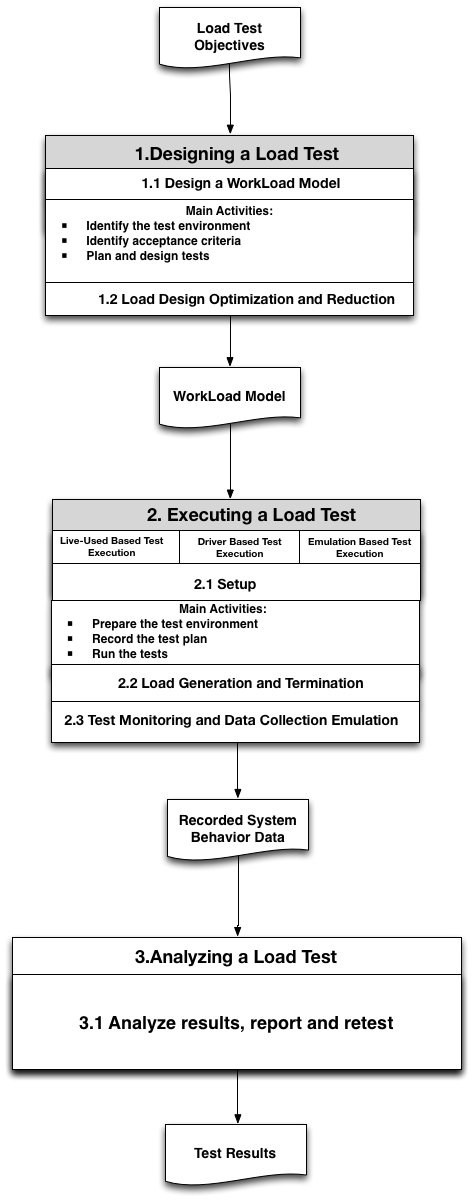
\includegraphics[width=0.5\textwidth]{./images/testprocess.png}
\caption{Load, Performance and Stress Test Process \cite{Jiang2010}\cite{Erinle2013}}
\label{fig:testprocess}
\end{figure}


The goal of the load design phase is to devise a load, which can uncover non-functional problems. Once the load is defined, the system under test executes the load and the system behavior under load is recorded. Load testing practitioners then analyze the system behavior to detect problems \cite{Jiang2010}. 

Once a proper load is designed, a load test is executed. The load test execution phase consists of the following three main aspects: (1) Setup, which includes system deployment and test execution setup; (2) Load Generation and Termination, which consists of generating the load; and (3) Test Monitoring and Data Collection, which includes recording the system behavior during execution\cite{Jiang2010}. 

The core activities in conducting an usual Load, Performance and Stress tests are \cite{Erinle2013}: 

\begin{itemize}
\item Identify the test environment: identify test and production environments and knowing the hardware, software, and network configurations helps derive an effective test plan and identify testing challenges from the outset.

\item Identify acceptance criteria: identify the response time, throughput, and resource utilization goals and constraints.

\item Plan and design tests:identify the test scenarios.In the context of testing, a scenario is a sequence of steps in an application. It can represent a use case or a business function such as searching a product catalog, adding an item to a shopping cart, or placing an order \cite{Corporation2007}.

\item Prepare the test environment: configure the test environment, tools, and resources necessary to conduct the planned test scenarios.

\item Record the test plan: record the planned test scenarios using a testing tool.

\item Run the tests: Once recorded, execute the test plans under light load and verify the correctness of the test scripts and output results.

\item Analyze results, report, and retest: examine the results of each successive run and identify areas of bottleneck that need addressing.  

\end{itemize}



\subsection{Automated Stress Test Tools}

Automated tools are needed to carry out serious load, stress, and performance testing. Sometimes, there is simply no practical way to provide reliable, repeatable performance tests without using some form of automation. The aim of any automated test tool is to simplify the testing process. Automated Test Tool  typically have the following components \cite{Molyneaux2009}:

\begin{itemize}
\item Scripting module: Enable recording of end-user activities in different middleware protocols;
\item Test management module: Allows the creation of test scenarios;
\item Load injectors: Generate the load with multiple workstations or servers;
\item Analysis module: Provides the ability to analyse the data collected by each test interation.
\end{itemize}

Apache JMeter is a free open source stress testing tool.  It has a large user base and offers lots of plugins to aid testing. JMeter is a desktop application designed to test and measure the performance and functional behavior of applications. The application it's purely Java-based and is highly extensible through a provided API (Application Programming Interface). JMeter works by acting as the client of a client/server application. JMeter allows multiple concurrent users to be simulated on the application \cite{Halili2008} \cite{Erinle2013}. 

JMeter has components organized  in a hierarchical manner. The Test Plan is the main component in a JMeter script. A typical test plan will consist of one or more Thread Groups, logic controllers, listeners, timers, assertions, and configuration elements:

\begin{itemize}
\item Thread Group: Test management module responsible to simulate the users used in a test. All elements of a test plan must be under a thread group.
\item Listeners: Analysis module responsible to provide access to the information gathered by JMeter about the test cases .
\item Samplers: Load injectors module responsible to send requests to a server, while Logical Controllers let you customize its logic.
\item Timers: allow JMeter to delay between each request.
\item Assertions: test if the application under test it is returning the correct results.
\item Configuration Elements: configure detais about the request protocol and test elements.
\end{itemize}


\subsection{Stress Test Results}

The system behavior recorded during the test execution phase needs to be analyzed to determine if there are any load-related functional or non-functional problems \cite{Jiang2010}.

There can be many formats of system behavior like resource usage data or end-to-end response time, which is recorded as response time for each individual request. These types of data need to be processed before comparing against threshold values.A proper data summarization technique is needed to describe these many data instances into one number. Some researchers advocate that the 90-percentile response time is a better measurement than the average/medium response time, as the former accounts for most of the peaks, while eliminating the outliers \cite{Jiang2010}.
